\documentclass[border={0pt 0pt 0pt 0pt}]{standalone}

\usepackage{hyperref}
\usepackage{tikz}
\usepackage{graphicx}

\usetikzlibrary{decorations.pathreplacing,
  arrows,
  calc,
  decorations.pathmorphing,
  decorations.pathreplacing,
  decorations.markings,
  positioning,
  shapes
}
\tikzstyle{snakearrow} = [decorate, decoration={pre length=0.1cm,
  post length=0.1cm, snake, amplitude=.4mm,
  segment length=4mm},thick, ->]

\ifpdf
% Ensure reproducible output
\pdfinfoomitdate=1
\pdfsuppressptexinfo=-1
\pdftrailerid{}
\hypersetup{
  pdfcreator={},
  pdfproducer={}
}
\fi

\begin{document}
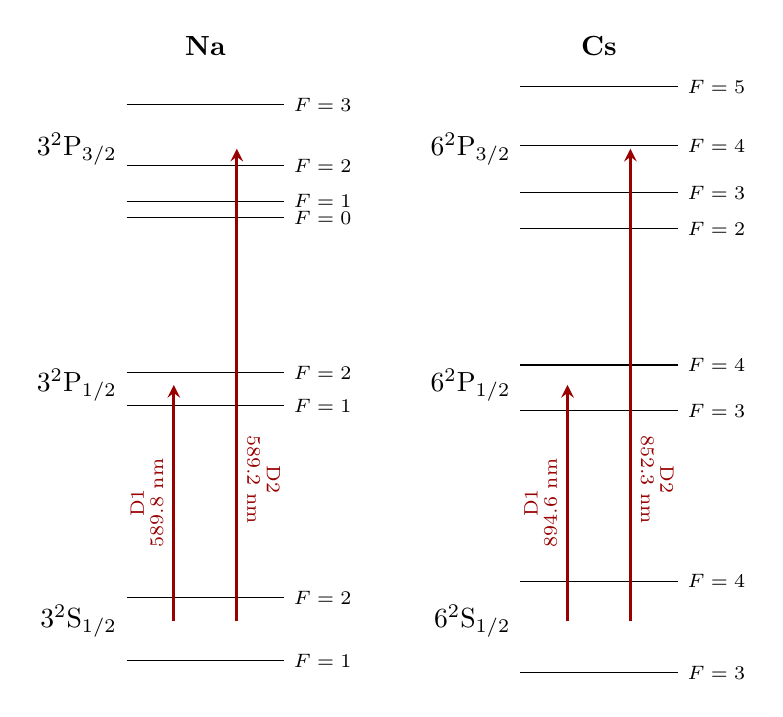
\begin{tikzpicture}
  \begin{scope}[shift={(-2.5, 0)}]
    \node at (0, 7.3) {\textbf{Na}};
    % ~6
    \draw (-1, 6 + 0.234 * 2.4) -- ++(2, 0) node[right] {\scriptsize $F=3$};
    \draw (-1, 6 - 0.088 * 2.4) -- ++(2, 0) node[right] {\scriptsize $F=2$};
    \draw (-1, 6 - 0.278 * 2.4) -- ++(2, 0) node[right] {\scriptsize $F=1$};
    \draw (-1, 6 - 0.366 * 2.4) -- ++(2, 0) node[right] {\scriptsize $F=0$};
    \node[left] at (-1, 6) {$3^2\mathrm{P}_{3/2}$};

    % ~3
    \draw (-1, 3 + 0.392 / 2.5) -- ++(2, 0) node[right] {\scriptsize $F=2$};
    \draw (-1, 3 - 0.653 / 2.5) -- ++(2, 0) node[right] {\scriptsize $F=1$};
    \node[left] at (-1, 3) {$3^2\mathrm{P}_{1/2}$};

    % ~0
    \draw (-1, 0 + 0.392 / 1.3) -- ++(2, 0) node[right] {\scriptsize $F=2$};
    \draw (-1, 0 - 0.653 / 1.3) -- ++(2, 0) node[right] {\scriptsize $F=1$};
    \node[left] at (-1, 0) {$3^2\mathrm{S}_{1/2}$};

    % D1/D2
    \draw[->,>=stealth,red!60!black,line width=1] (-0.4, 0) --
    node[above,rotate=90,align=center,execute at begin node=\setlength{\baselineskip}{7pt}]
    {\scriptsize D1\\\scriptsize$589.8~\mathrm{nm}$} (-0.4, 3);

    \draw[->,>=stealth,red!60!black,line width=1] (0.4, 0) --
    node[above,pos=0.3,rotate=-90,align=center,execute at begin node=\setlength{\baselineskip}{7pt}]
    {\scriptsize D2\\\scriptsize$589.2~\mathrm{nm}$} (0.4, 6);
  \end{scope}

  \begin{scope}[shift={(2.5, 0)}]
    \node at (0, 7.3) {\textbf{Cs}};
    % ~5
    \draw (-1, 6 + 0.262 * 3.0) -- ++(2, 0) node[right] {\scriptsize $F=5$};
    \draw (-1, 6 + 0.013 * 3.0) -- ++(2, 0) node[right] {\scriptsize $F=4$};
    \draw (-1, 6 - 0.187 * 3.0) -- ++(2, 0) node[right] {\scriptsize $F=3$};
    \draw (-1, 6 - 0.338 * 3.0) -- ++(2, 0) node[right] {\scriptsize $F=2$};
    \node[left] at (-1, 6) {$6^2\mathrm{P}_{3/2}$};

    % ~3
    \draw (-1, 3 + 0.508 / 2) -- ++(2, 0) node[right] {\scriptsize $F=4$};
    \draw (-1, 3 - 0.654 / 2) -- ++(2, 0) node[right] {\scriptsize $F=3$};
    \node[left] at (-1, 3) {$6^2\mathrm{P}_{1/2}$};

    % ~0
    \draw (-1, 0 + 0.508) -- ++(2, 0) node[right] {\scriptsize $F=4$};
    \draw (-1, 0 - 0.654) -- ++(2, 0) node[right] {\scriptsize $F=3$};
    \node[left] at (-1, 0) {$6^2\mathrm{S}_{1/2}$};

    % D1/D2
    \draw[->,>=stealth,red!60!black,line width=1] (-0.4, 0) --
    node[above,rotate=90,align=center,execute at begin node=\setlength{\baselineskip}{7pt}]
    {\scriptsize D1\\\scriptsize$894.6~\mathrm{nm}$} (-0.4, 3);

    \draw[->,>=stealth,red!60!black,line width=1] (0.4, 0) --
    node[above,pos=0.3,rotate=-90,align=center,execute at begin node=\setlength{\baselineskip}{7pt}]
    {\scriptsize D2\\\scriptsize$852.3~\mathrm{nm}$} (0.4, 6);
  \end{scope}
\end{tikzpicture}
\end{document}
